% !TeX spellcheck = en_GB
\documentclass[a4paper,12pt]{article}

\usepackage{anysize}
\marginsize{30mm}{20mm}{20mm}{20mm}
\usepackage[utf8]{inputenc}
\usepackage[english]{babel}
\usepackage[style=ieee,backend=biber,sorting=none]{biblatex}
\addbibresource{FinalReport.bib}
\usepackage{amsmath}
\usepackage{graphicx}
\graphicspath{ {./generatedImages/} }
\usepackage{svg}
\usepackage{setspace}
\singlespacing
\parskip 0ex 
\usepackage{array}
\newcolumntype{L}{>{\centering\arraybackslash}m{100mm}}
\newcolumntype{M}{>{\centering\arraybackslash}m{50mm}}


%opening
\title{Linear Direct Current Electromagnetic Motor with Liquid Eutectic Gallium-Indium Alloy Coil}
\author{Jason Guan}
\date{27 September 2019}
\begin{document}
\maketitle
\begin{center}
	892594255\\
	Department of Engineering Science\\
	Supervised by Dr. Bryan Ruddy
\end{center}

\newpage

\begin{abstract}
Abstract placeholder
\end{abstract}

\newpage

\section*{Acknowledgements}
Paul Roberts 

Steve Oldman 

Greg  

Nick, Suroosh, Mahsa and Yahya 

And of course, Dr. Bryan Ruddy 

\newpage

\tableofcontents

\newpage

\section{Table of Notation}
\begin{center}
	\begin{tabular}{c | L | c} 
		\textbf{Symbol} & \textbf{Description} & \textbf{Units} \\ [0.5ex] 
		\hline\hline
		$P_{in}$ & Electrical power input & $W$ \\ 
		\hline
		$P_{out}$ & Total power output & $W$ \\ 
		\hline
		$P_{mech}$ & Mechanical power output & $W$ \\ 
		\hline
		$P_{heat}$ & Heat power output & $W$ \\ 
		\hline
		$f$ & Frequency & $Hz$ \\ 
		\hline
		$\mathcal{F}$ & Magnetomotive force & $A$ \\ 
		\hline
		$\mathcal{R}$ & Magnetic reluctance & $H^{-1}$ \\ 
		\hline
		$\mathcal{R}_{mag}$ & Magnetic reluctance of the magnet & $H^{-1}$ \\ 
		\hline
		$\Phi$ & Magnetic flux & $Wb$ \\ 
		\hline
		$\Phi_0$ & Short circuit magnetic flux, i.e. flux in circuit when poles of magnet are connected with minimal reluctance & $Wb$ \\ 
		\hline
		$L_{Wtotal}$ & Total length of wire in motor & $m$ \\
		\hline
		$L_{mag}$ & Axial length of cylindrical magnet & $m$ \\
		\hline
		$B$ & Magnetic field density & $T$ \\
		\hline
		$B_{r}$ & Residual flux density of magnet & $T$ \\
		\hline
		$I$ & Electric current & $A$ \\
		\hline
		$d_{travel}$ & Required travel distance of the motor bobbin & $m$ \\
		\hline
		$c_{pWire}$ & Specific heat capacity of wire & $JKg^{-1}K^{-1}$ \\
		\hline
		$\mu_0$ & Vaccum permeability, $4\pi\times10^{-7} Hm^{-1}$ \cite{engineeringtoolboxPermeability2016} & $Hm^{-1}$ \\
		\hline
		$\mu_s$ & Relative magnetic permeability of mild steel, 760 \cite{baartmanMaterialsLibraryFEMM2007} & NA \\
		\hline
		$\mu_m$ & Relative magnetic permeability of neodymium magnet, 1.05 \cite{engineeringtoolboxPermeability2016} & NA \\
		\hline
	\end{tabular}
\end{center}

\newpage

\section{Introduction}
Background\\

Soft robots important \\

Methods of locomotion all new, each with different advantages and drawbacks \\

Lack of traditional locomotion options \\

Liquid metal wired electromagnetic motors presents a possible solution \\

Transferral of existing robotics locomotion corpus to soft robots \\

Also presents a possible advantage re: cooling by circulating the wires \\

Question Statement \\

Is it feasible to build an electromagnetic motor using liquid metal for wiring that can also be cooled via circulating metal in the wiring? \\

Aims \\

Design, build and characterise an electromagnetic motor with liquid metal coils\\

\newpage

\section{Design, Manufacturing and Assembly}
\subsection{Mathematical Modelling}
\subsubsection{Motor Force}

\begin{equation} \label{eq:emmfdef}
\mathcal{F}=\mathcal{R} \Phi
\end{equation}
Magnetomotive force of a magnet can be calculated using total magnetic reluctance in a magnetic circuit and magnetic flux in that circuit, seen in equation \ref{eq:emmfdef}. This is analogous to electrical circuits following Ohm's law: magnetomotive force is analogous to voltage, reluctance is analogous to resistance and flux is analogous to current. Magnetomotive force in cylindrical magnets can be calculated using a short circuit scenario, i.e. by assuming poles of magnet are connected with minimal reluctance. Under the assumption that magnetic field density is uniform, the short circuit flux is equal to the remanence field density of the magnet multiplied by the cross-sectional area of the magnet normal to the direction of the magnetic field. In the case of an axially magnetised cylindrical magnet, this area is equal to the radial cross-section area of the cylinder.
\begin{equation}\label{eq:shortflux}
\Phi_0 = B_rA_{mag}
\end{equation}
Substituting equation \ref{eq:shortflux} into equation \ref{eq:emmfdef} gives a way to simply calculate $\mathcal{F}$ using axial length of magnet and remanent field density:
\begin{equation}\label{eq:emmf1}
\begin{split}
\mathcal{F} & = \mathcal{R}_{mag} \Phi_0\\
& = \frac{L_{mag}}{A_{mag}}B_r A_{mag}\\
& = L_{mag} B_r
\end{split}
\end{equation}
The magnetic circuit of a voice coil motor travels through four components in series: the magnet, the core, the "air" gap where the coils are and the shell, seen in figure \ref{fg:simplemotor}.
\begin{figure}[h] \label{fg:simplemotor}
	\centering
	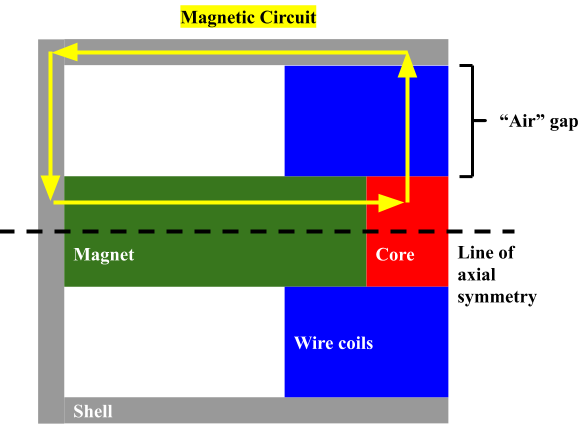
\includegraphics[scale=0.4]{simplifiedMotor.png}
	\caption{Simplified axisymmetric diagram of typical moving-wire voice coil motor}
\end{figure}
This means the total reluctance in the circuit can be represented by equation \ref{eq:rttl}, similar to how resistance is calculated in an electrical circuit.
\begin{equation}\label{eq:rttl}
\mathcal{R}_{total}=\mathcal{R}_{gap}+\mathcal{R}_{mag}+\mathcal{R}_{core}+\mathcal{R}_{shell}
\end{equation}
Magnetic reluctance can be calculated as the proportion of magnetic path length $l_m$ and the product of material permeability $\mu$ and cross-sectional area normal to magnetic flux $A$, seen in equation \ref{eq:rcalc} \cite{coatesTransformerCoresReluctance2018}.
\begin{equation}\label{eq:rcalc}
\mathcal{R}=\frac{l_m}{\mu A}
\end{equation}
Assuming the shell and core are made out of magnetically conductive material such as mild steel, the permeability of shell and core will be hundreds of times higher than the permeability of "air" gap and magnet \cite{engineeringtoolboxPermeability2016}. Therefore, the reluctance of shell and core can be approximated to zero for the purposes of this calculation. 
Substituting simplified equation \ref{eq:rttl} into equation \ref{eq:emmfdef} produces:
\begin{equation}\label{eq:emmfreal}
\mathcal{F}=(\mathcal{R}_{gap}+\mathcal{R}_{mag})\Phi
\end{equation}
Reluctance between two coaxial cylinders, in this case between the magnet and the shell, can be calculated as in equation \ref{eq:rgap}, assuming all magnetic flux flows through the core \cite{changChapterElectrodynamics2006}. Relative permeability of the gap is approximated to 1 as none of air, silicone or eGaIn are ferromagnetic \cite{engineeringtoolboxPermeability2016}.
\begin{equation}\label{eq:rgap}
\mathcal{R}_{gap}=\frac{\mu_0 \ln{\frac{r_{out}}{r_{in}}}}{2\pi L_{core}}
\end{equation}
Reluctance through the magnet can be calculated as seen in equation \ref{eq:rmag}, similar to how resistance would be calculated for a cylinder.
\begin{equation}\label{eq:rmag}
\mathcal{R}_{mag}=\frac{\mu_m L_{mag}}{2\pi r_{mag}^2}
\end{equation}
Substituting equations \ref{eq:rgap}, \ref{eq:rmag} and \ref{eq:emmf1} into equation \ref{eq:emmfreal} gives equation \ref{eq:emmfsubbed} which yields flux in the motor magnetic circuit.
\begin{equation}\label{eq:emmfsubbed}
\begin{split}
L_m B_r & = \frac{\ln{\frac{r_{out}}{r_{in}}}}{2\pi L_c}\Phi\\
\frac{2\pi L_m L_c B_r}{\ln{\frac{r_{out}}{r_{in}}}} & = \Phi\\
\end{split}
\end{equation}
To calculate the magnetic field density in the "air" gap, which can then be used to calculate force acting on the moving coils, the area of action that the flux is distributed across is also required as seen in equation \ref{eq:fluxdef}.
\begin{equation}\label{eq:fluxdef}
\Phi = B_{gap}A_{active}
\end{equation}
Substituting equation \ref{eq:fluxdef} into equation \ref{eq:emmfsubbed} gives equation \ref{eq:fluxsubbed}, which can be used to calculate the magnetic field density $B_{gap}$ across the "air" gap.
\begin{equation}\label{eq:fluxsubbed}
B_{gap} = \frac{2\pi L_{mag} L_{core} B_r}{\ln{\frac{r_{out}}{r_{in}}}A_{active}}
\end{equation}
Using Lorentz's force law substituted with equation \ref{eq:fluxsubbed}, equation \ref{eq:fbil} gives a minimum current $I$ can be obtained given a known required force $F$ and a known length of wire in the magnetic field $L_{active}$.
\begin{equation}\label{eq:fbil}
\begin{split}
F & = B_{gap}IL_{active}\\
I & = \frac{F}{B_{gap}L_{active}}\\
I & = \frac{F A_{active} \ln{\frac{r_{out}}{r_{in}}}}{2\pi L_{mag} L_{core} B_r L_{active}}
\end{split}
\end{equation}
The active area in the magnetic field is different for each layer of wire in the motor. Layers of wire further away from the magnet, meaning a larger area and therefore lower magnetic field density. The total active area that magnetic flux is distributed across can be calculated as shown in equation \ref{eq:activearea}, where $n$ is the total number of wire layers.
\begin{equation}\label{eq:activearea}
A_{active} = \sum_{1}^{n}{A_{active}^{layer}} = 2\pi L_c (r_{core}-r_{wireout} + 2r_{wireout} \frac{(n+1)n}{2})
\end{equation}
The length of wire in the magnetic field can be calculated in a similar fashion, shown in equation \ref{eq:activel}.
\begin{equation}\label{eq:activel}
L_{active} = L_{core}\pi(layers+1)layers + \frac{L_{core} r_{mag} \pi}{r_{wireOut}}
\end{equation}
Combining equations \ref{eq:fbil}, \ref{eq:activearea} and \ref{eq:activel} yields a final current calculation in equation \ref{eq:finalcurrent}.
\begin{equation}\label{eq:finalcurrent}
I = \frac{F\cdot 2\pi L_c (r_{core}-r_{wireout} + 2r_{wireout} \frac{(n+1)n}{2}) \ln{\frac{r_{out}}{r_{in}}}}{2\pi L_{mag} L_{core} B_r L_{core}\pi(layers+1)layers + \frac{L_{core} r_{mag} \pi}{r_{wireOut}}}
\end{equation}

\subsubsection{Heat and Temperature}
Using heat energy can calculate temperature in wires
Safety

\begin{figure}[h] \label{fg:motorheat}
\centering
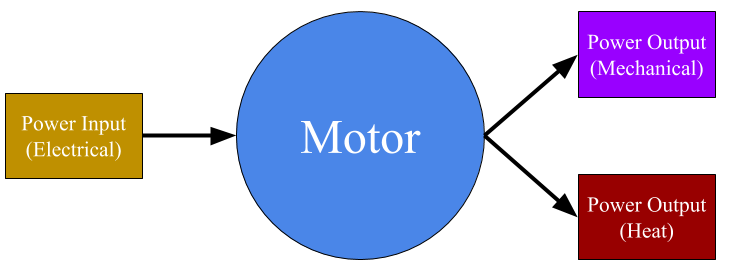
\includegraphics[scale=0.4]{motorheat.png}
\caption{Conservation of energy in the motor system}
\end{figure}

\begin{equation}\label{eq:pin}
P_{in} = IV = I^2R
\end{equation}

\begin{equation}\label{eq:resistance}
R=\frac{L_{Wtotal}}{A\sigma}
\end{equation}

\begin{equation}\label{eq:pbreakdown}
P_{in}=P_{out}=P_{mech}+P_{heat}
\end{equation}

\begin{equation}\label{eq:pmechbreakdown}
\begin{split}
P_{mech} & = \vec{F}\vec{d}\\
& = BIL\cdot d_{travel} \cdot f
\end{split}
\end{equation}

Combining equations \ref{eq:pin}, \ref{eq:resistance}, \ref{eq:pbreakdown} and \ref{eq:pmechbreakdown} gives a formulation for temperature change of wires, assuming heat energy is conserved in wires:

\begin{equation}\label{eq:pheatbreakdown}
\begin{split}
P_{heat} & = P_{in}-P_{mech}\\
\rho Q c_{pWire} \Delta T & = \frac{I^2L_{Wtotal}}{A\sigma}-BIL\cdot d \cdot f \\
\Delta T & = \frac{\frac{I^2L_{Wtotal}}{A\sigma}-BIL\cdot d \cdot f}{\rho Q c_{pWire}}
\end{split}
\end{equation}


\subsection{Optimisation Algorithm}
\begin{figure}[h] \label{fg:optiAlgo}
	\centering
	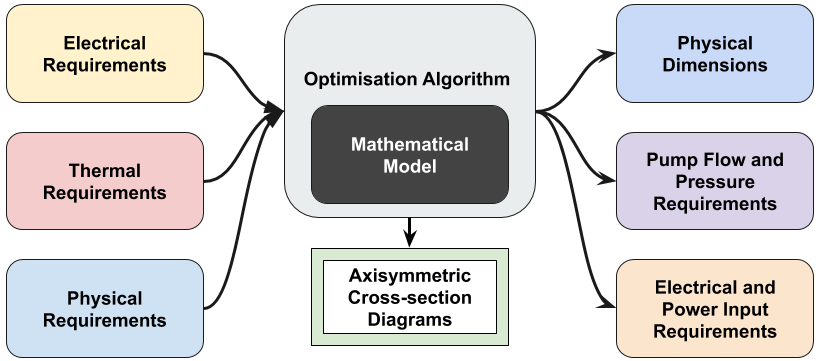
\includegraphics[scale=0.4]{optiAlgro.png}
	\caption{Diagrammatic representation of optimisation algorithm inputs and outputs}
\end{figure}

Grid-search optimisation for even numbered layers.

Optimised for an optimisation variable $\mathcal{P}$, which is the product of total motor mass and electrical input power.

Runs requirement checking function on each result and discards invalid solutions.

\begin{center}
	\begin{tabular}{M | M | M} 
		\textbf{Variable} & \textbf{Requirement} & \textbf{Justification} \\ [0.5ex] 
		\hline\hline
		Output force & Must be over 9 N & Minimum to drive liquid metal pump \\
		\hline
		Acceptable temperature change in wires & Must be under 30 K & Higher temperatures may be a health and safety hazard \\
		\hline
		Travel distance of motor & Must be over 9 mm & Minimum to drive liquid metal pump \\ 
		\hline
		Bobbin length & Must be shorter than combined length of core and magnet & Not physically valid otherwise \\ 
		\hline
		Shell internal diameter & Must be under 80 mm & Not practical for manufacturing, assembly and handling if bigger \\ 
		\hline
		Circuit current & Must be under 10 A & No power supply available to drive more than 10 A \\ 
		\hline
		Total volume of wire & Must be under 15 ml & Limit to amount of eGaIn available and difficult to assemble with larger volume \\ 
		\hline
		Flow rate of liquid metal in wires & Must be positive & Validity check \\ 
		\hline
		Electrical power input & Must be positive & Validity check \\ 
		\hline
	\end{tabular}
\end{center}

Optimisation was conducted assuming the use of 2 mm internal diameter, 3 mm external diameter silicone tubing for wiring. This was the tubing with largest internal volume to total volume ratio that was commercially available.

The optimisation software produced physical dimensions, pump flow and pressure requirements, electrical input requirements and an axisymmetric cross-section diagram to show scale of the optimised motor for each number of layers that the optimisation was run for.

\begin{center}
	\begin{tabular}{M | c | c | c} 
		\textbf{Variable} & \textbf{4-layer solution} & \textbf{6-layer solution} & \textbf{Units} \\ [0.5ex] 
		\hline\hline
		Magnet length & 35 & 42.5 & $mm$ \\ 
		\hline
		Magnet radius & 20 & 20 & $mm$ \\ 
		\hline
		Core length & 12 & 8 & $mm$ \\ 
		\hline
		Bobbin length & 27.5 & 23.75 & $mm$ \\ 
		\hline
		Shell internal radius & 33.5 & 39.5 & $mm$ \\ 
		\hline
		Total wire length & 6.68 & 9.55& $m$ \\ 
		\hline
		Total wire resistance & 0.15 & 0.22 & $\Omega$ \\ 
		\hline
		Minimum required current & 7.75 & 6.27 & $A$ \\ 
		\hline
		Minimum required voltage & 1.19 & 1.38 & $V$ \\ 
		\hline
		Minimum power input & 9.22 & 8.63 & $W$ \\ 
		\hline
		Flow rate required for circulation cooling & 0.135 & 0.125 & $ml\cdot s^{-1}$ \\ 
		\hline
		Pressure required to drive circulation cooling & 5.51 & 7.28 & $kPa$ \\ 
		\hline
		Total mass of motor & 1.21 & 1.50 & $kg$ \\ 
		\hline
		Optimisation Variable $\mathcal{P}$ & 11.19 & 12.98 & $kg\cdot W$ \\ 
		\hline
	\end{tabular}
\end{center}

Choice between 4 layer design and 6 layer design

\begin{figure}[h] \label{fg:finalmotor}
	\centering
	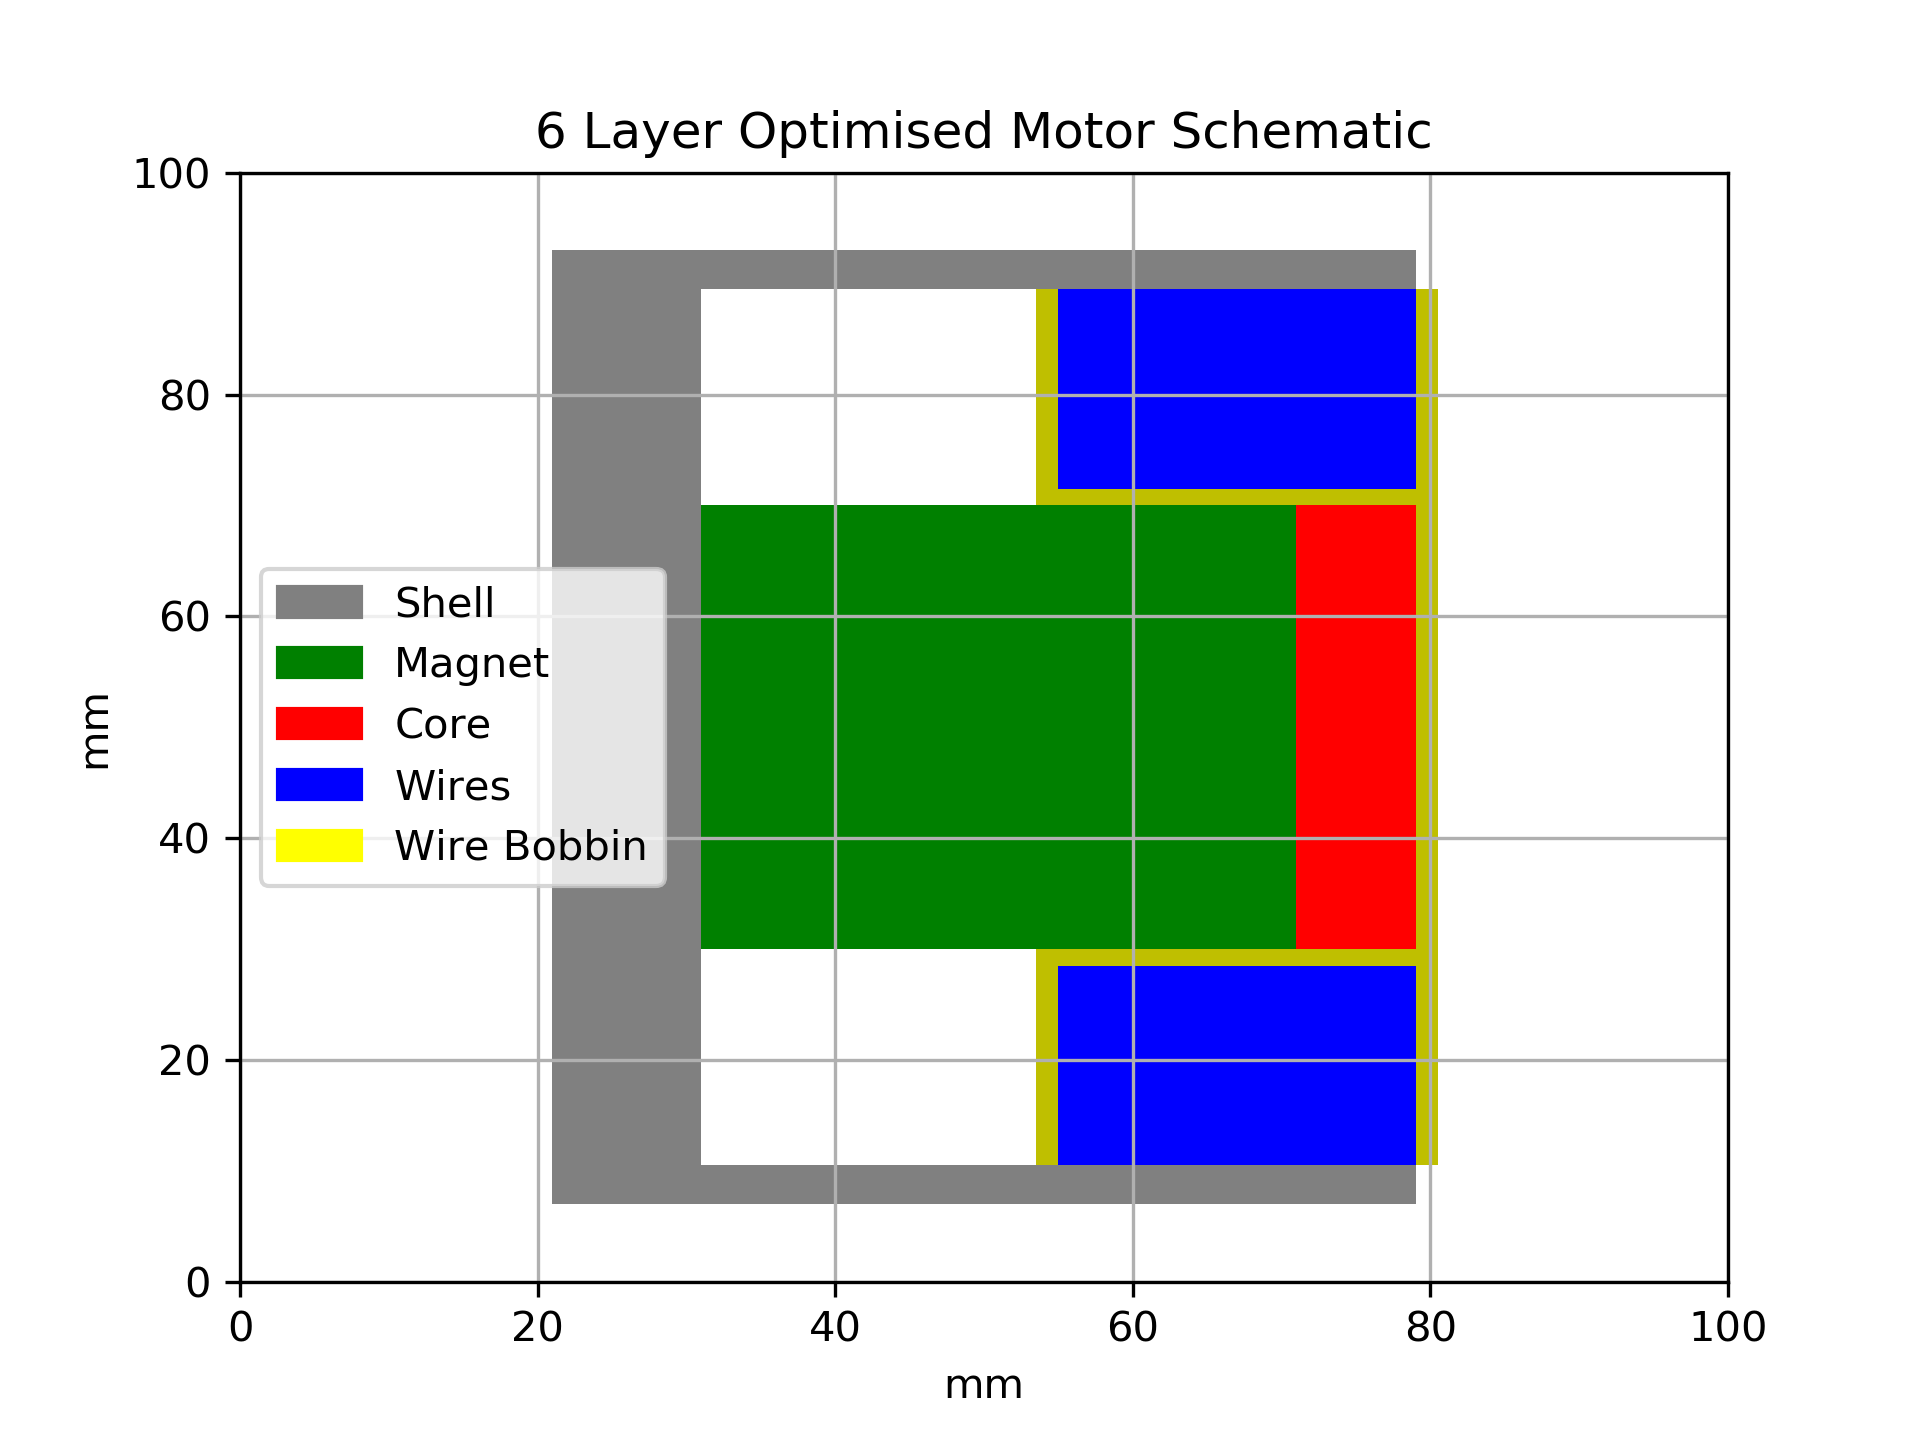
\includegraphics[scale=0.5]{finalDesign_layers.png}
	\caption{Graphical representation of cross-section of final motor design}
\end{figure}

\subsection{Design Validation}
Abacus Maxwell 2D axisymmetric electromagnetic simulation

\subsection{Physical Design and Manufacturing}
4 axial, 40 mm diameter, 10 mm tall N45 grade neodymium disc magnets were used in series, to substitute for the required 40 mm diameter, 42.5 mm tall N42 grade neodymium magnet. The disc magnets also come with countersunk unthreaded M6 holes for fastening. 

\subsubsection{Shell}



\subsubsection{Core}

\subsubsection{Wire Bobbin}

\subsection{Assembly}

\subsubsection{Shell and Magnet Assembly}

\subsubsection{Wire Assembly}

\subsubsection{Health, Safety and Containment}

\newpage

\section{Experiment Designs and Results}

\subsection{Experiment 1: Force Characterisation}

\subsubsection{Method}

\subsubsection{Results}

\subsection{Experiment 2: Circulation Thermoregulation}

\subsubsection{Method}

\subsubsection{Results}

\newpage

\section{Discussion}

Application to the original physical situation\\ 

Comparison with related problems and other solutions\\

Critical assessment of significance\\

Difficulty of the problem and how well it has been tackled\\

\cite{liuLiquidMetalMachine2016}

\newpage

\section{Conclusion}

\newpage

\section{Appendices}

\newpage
References to previous works should be made in a consistent way. Specific references should be itemised in the Reference list, with any other more general material listed in a Bibliography. Only those books and papers actually consulted should be included. There are several variations on layout of reference lists; obtain advice from your supervisor and the library staff.  

\printbibliography
	
\end{document}
